	
\documentclass[twocolumn]{autart}    % Enable this line and disable the 
                                     % preceding line to obtain a two-column 
                                     % document whose style resembles the
                                     % printed Automatica style.
                                     

\usepackage{hyperref}

\usepackage{graphicx}          % Include this line if your 
                               % document contains figures,
%\usepackage[dvips]{epsfig}    % or this line, depending on which
                               % you prefer.

\begin{document}

\begin{frontmatter}
%\runtitle{Insert a suggested running title}  % Running title for regular 
                                              % papers but only if the title  
                                              % is over 5 words. Running title 
                                              % is not shown in output.

\title{Dota Team Builder\thanksref{footnoteinfo}} % Title, preferably not more 
                                                % than 10 words.

\thanks[footnoteinfo]{$https://drive.google.com/open?id=0B_Gei_HEl-WgSEVScXRmLTUyOGM$}
							
\author{Narmamatov Kadyrbek}
\ead{kadirpili@gmail.com} 

\address{South Korea, UNIST} 

          
\begin{keyword}                             
Dota2; Recommendation Tool; Game helper.             
\end{keyword}                             

\begin{abstract}                          	
Dota Team Builder (DTB) is aimed to help Dota2 gamers to choose a good playing hero against enemy team. Unlike traditional recommendation tools, DTB provides a nice and easy to use interface and most importantly gives to user a chance to compare recommended heroes between each other and decide the final choice. It gives a user insights in choosing a hero by visualization frameworks as stacked/grouped chart and gauge indicators.   

\end{abstract}

\end{frontmatter}

\section {INTRODUCTION}

\subsection{INTRODUCTION OF DOTA2}
	Dota2 is a world wide played game, which has a user-base of up to 10 millions nowadays. The most played and original of Dota2 mode is 'All Pick' mode, which will be explained in details later. In this mode a game consists of 2 teams(teams are called Radiant and Dire), located on opposite corners of the map. The green team located on the bottom left(Radiant), while red team located on the top right corner (Dire). 
 The main goal of each team is to attack and destroy the main building of enemy team. Each team has 5 players and each player has to choose a hero out of 112 heroes and controls it, focusing on leveling up that hero. Each hero has its own characteristics and abilities. 
A purpose of game is very simple, but the game itself not so easy. To become a good player, you should spent a lot of time practising with good players and learning game tips. There is a big community of dota gamers now, and still there is a big flow of new comers to the world of dota2. 


\begin{figure}
\begin{center}
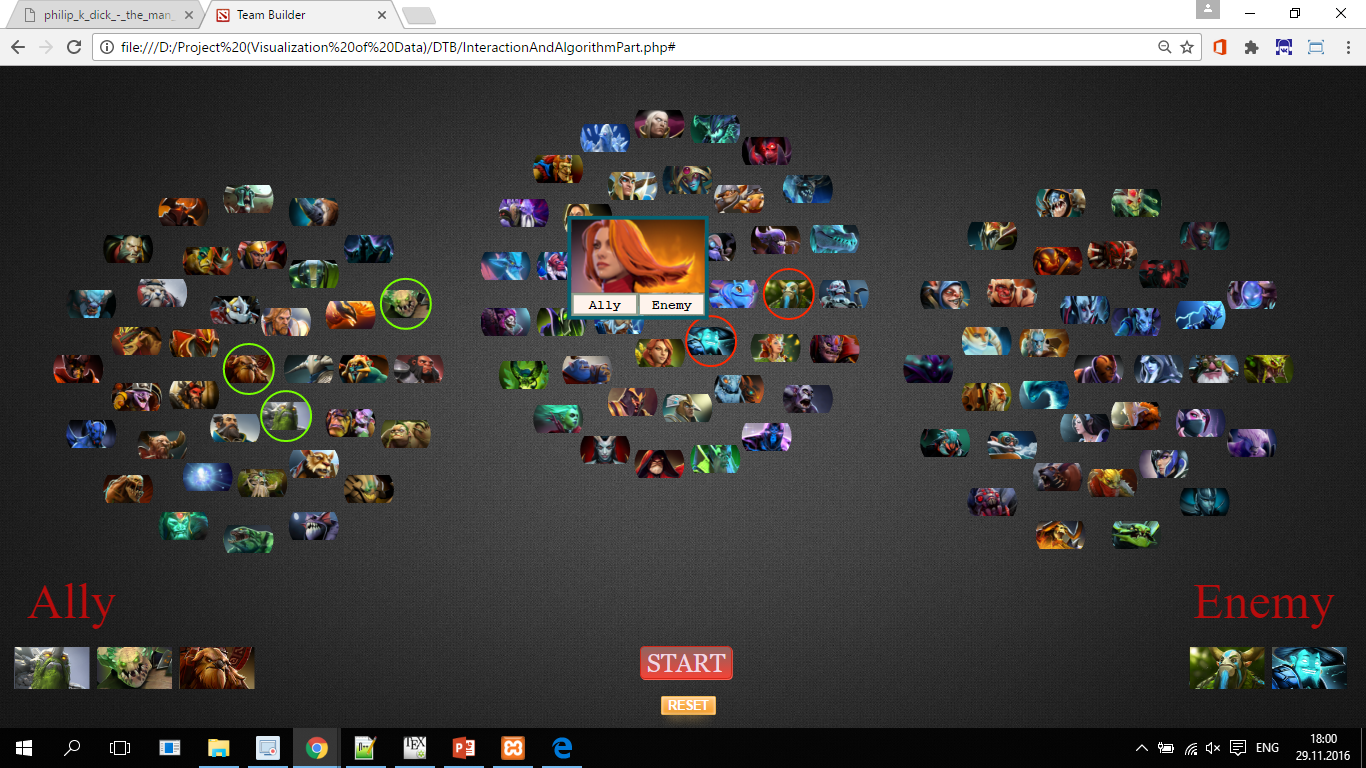
\includegraphics[height=4cm]{herochoosing.png}    % The printed column  
\caption{Hero Choosing Interface}  % width is 8.4 cm.
\label{herochoosing}                                 % Size the figures 
\end{center}                                 % accordingly.
\end{figure}



\subsection{MOTIVATION} It is well known among players that to be a strong team you do not have to have a collection of the strongest or the best heroes but you must consider how a heroes can help each other and be effective against enemy team. But how do players know which hero to choose to be effective? Let me explain 3  techniques that players usually use when choosing a hero:

1. Experience - most powerful thing to use. For example, if you have played a 100 games against 'Zeus' before, you will probably know which player will be good against 'Zeus' now. if you have played 1000 games against 'Zeus', it will be more probably that you will choose the most optimal hero against him. Most used by professionals, obviously.   

2. Logic. For example, if you know that your enemy chosen 'Rikimaru' which can be invisible and its his most important ability. Then you will probably choose 'Silencer' which has an ability to show invisible heroes for a while, but it can not be always good reason to rely.  
	3. Recommendation tools. There some websites and mobile application that offer heroes to choose in your situation. For example, if you know that 2 of your enemies already chosen heroes and 4 of your allies also chosen heroes(number of heroes does not matter), these applications shows you some heroes to choose, which is considered to be an optimal heroes, but it is not known how do their apps work to predict optimal heroes.

My idea is to provide a new recommendation tool with an easy and convenient interface and in which a player is able to compare and choose a hero among offered heroes.

\begin{figure}
\begin{center}
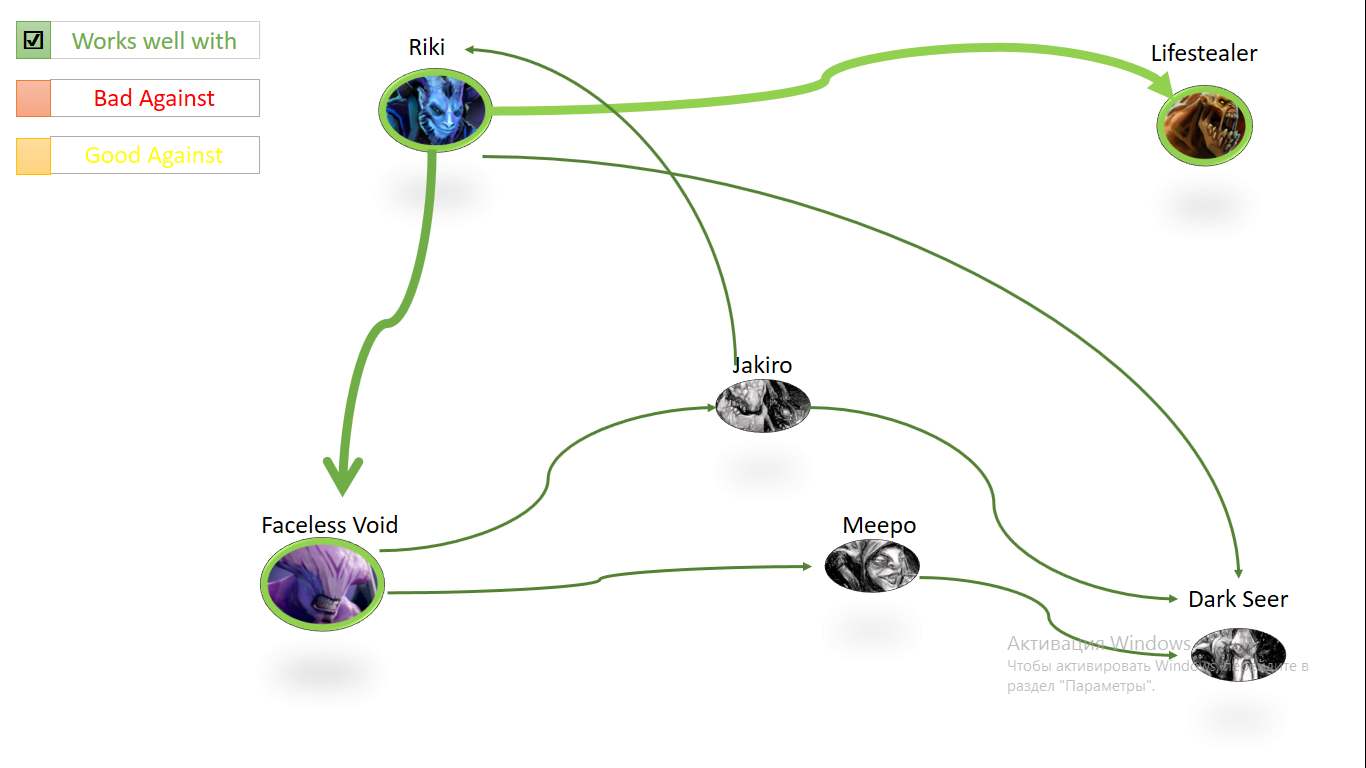
\includegraphics[height=4cm]{firstidea.png}    % The printed column  
\caption{Static sample visualization with edged graph}  % width is 8.4 cm.
\label{firstidea}                                 % Size the figures 
\end{center}                                 % accordingly.
\end{figure}



\section{RELATED WORK}
I found 6 websites and 2 apps similar to my project. The main purpose of them was same, but how did they approached to it and how did they showed data was different. Let's see what are they and how they are:

1. \href{http://www.dotateam.me/}{dotateam.me}. A user chooses a collection of only \emph{ally} heroes and app suggests 5 top most optimal heroes and also gives an advice which type of hero to choose. Makes a \emph{Win Rate vs. Game Duration} graph for chosen heroes.

2. \href{http://www.dotaedge.com/}{dotaedge.com}. Very simple and easy to understand app which gives an ability to choose an \emph{ally} team and returns a list of counters of 5 types[great,good,ok,avoid picking].  

3. \href{https://dota2.becomethegamer.com/dashboard}{dota2.becomethegamer.com}. Gives a huge amount of data about recommended heroes. Gives ability to choose both \emph{ally} and \emph{enemy} team. It is the best tool in my opinion nowadays which provides a lot of information to help to conclude your choice. 

\emph{Here we see that first two recommendation  websites only provide a user to select only ally teams, which I think, main disadvantage, whereas third one provides both ally and enemy team selection. Let's see $3^{rd}$ tool which has in itself all main functions of other recommendation tools and compare  that to my project. First difference is that my visualization project provides detailed information about hero and shows top 20 heroes to choose. There are many differences in design but the main differences in ideas is providing an information to help a user to choose by himself in easy and convenient way. 
Here are only three recommendation tools explained, 4 others are almost with same characteristics. It could be said that my project is a combination of these three apps. }


There also many works related to dota2 issues and I referred to some of them in this paper. Here an explanation of some of the previous works:

1. \href{http://cs229.stanford.edu/proj2013/PerryConley-HowDoesHeSawMeARecommendationEngineForPickingHeroesInDota2.pdf}{How Does He Saw Me?} This paper explains a method to recommend a hero by machine learning and to get the probability of team's won. Though I did not use any machine learning, I used methodology part to understand how I can apply my own algorithm and to know why it could function correctly.

2. \href{https://classes.soe.ucsc.edu/cmps161/Winter14/projects/athsueh/proj/projectReport.pdf}{Dotabase: a Dota 2 Database Visualizer}
Author of this paper provides a visualization in 3D scatter plot and star plot by analysing gamer's previous played games. A player can enter queried matches in order to observe an informative and 					
educational representation of their statistics. A 3D scatter plot: displaying multiple heros’ performance for a player. A star plot: show the roles of a player, and their performance for each respective role. So the main goal is to improve player's weaknesses by showing him/her statistics about previous played games. 

3. \href{http://web.stanford.edu/class/archive/cs/cs448b/cs448b.1166/cgi-bin/wiki/images/a/ae/Cqiaoben_final.pdf}{Visualizing Match up Matrix}  This paper is about visualization which allows user to perform comparison between each individual by organizing data in meaningful
patterns. The whole visualization generation process is automated.

I used the partial ideas of above papers to improve my project.  

\begin{figure}
  \centering
  
    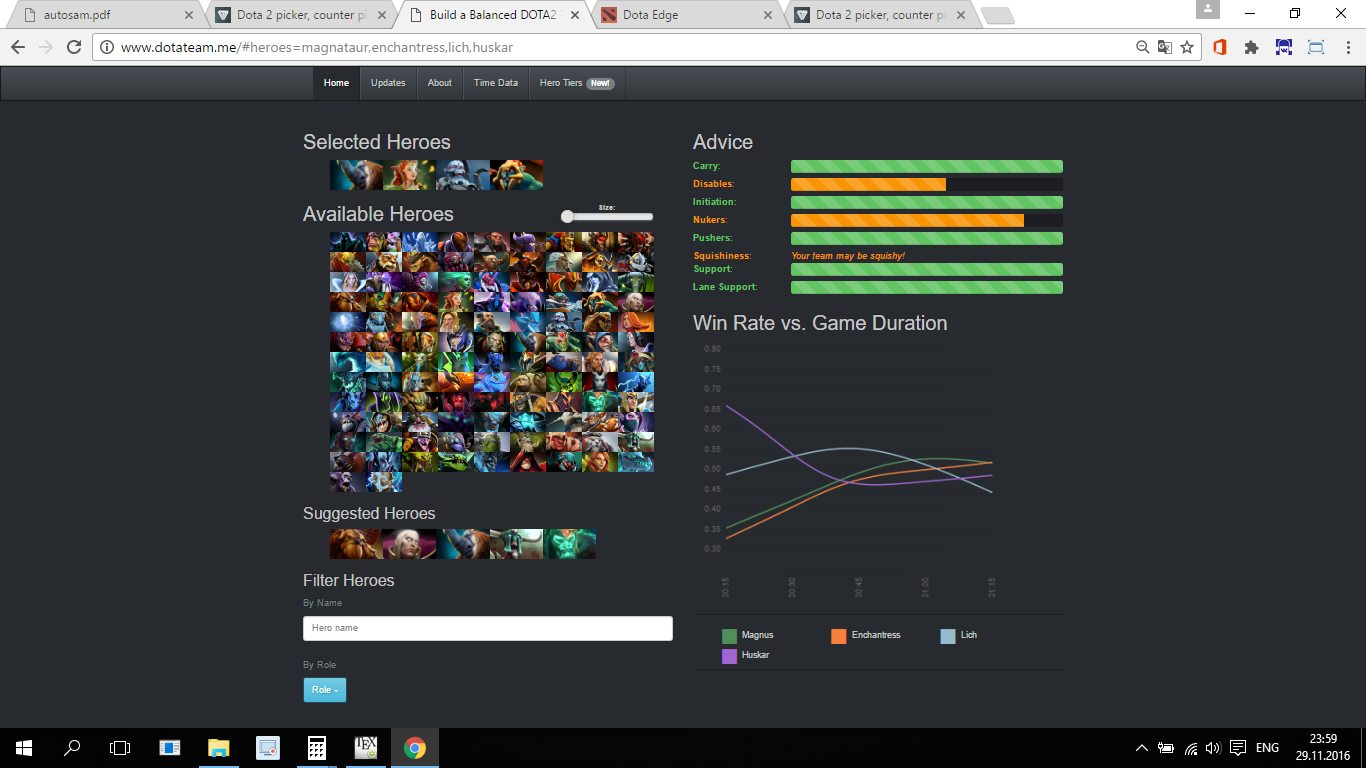
\includegraphics[width=0.5\textwidth]{dotateam.png}
\caption{http://www.dotateam.me/}
 \label{dotateam}
 
\end{figure}

\begin{figure}
\begin{center}
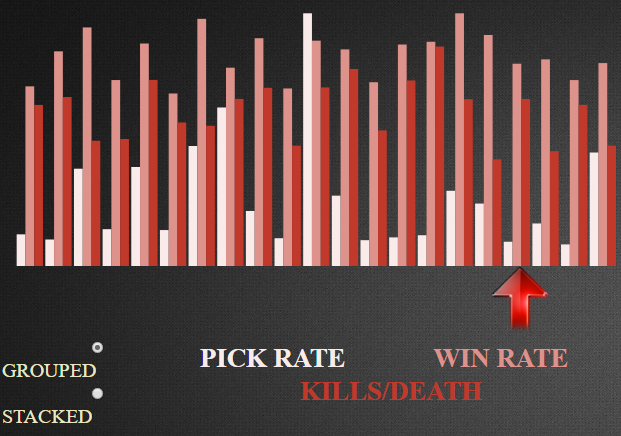
\includegraphics[height=4cm]{grouped.png}    % The printed column  
\caption{Grouped bar from stacked.}  % width is 8.4 cm.
\label{grouped}                                 % Size the figures 
\end{center}                                 % accordingly.
\end{figure}


\section{DATA SET}
I used Valve's Steam API to retrieve data about recently played games. Since not every match could be properly  analysed, I used some criteria for my data:

	1. Game Mode - All Pick. Most played mode of all. This game mode is the closest
to the true vision of Dota2 and it is not obvious to generalize other modes to my data analyses part. 

	2. Skill level - 'very high'. I used this criteria to see every hero shown up in their full potential in match while played by very high skilled players. 

	3. Number of heroes - 10

	4. Leave status - No one leaves game until it finished. Such matches do not capture how the absent
players' heroes affect to the outcome of the match.		

	5. Duration of game is greater than 900 seconds(or 15 minutes)



The data of all retrieved matches are stored in JSON file, which contains following information of each hero for my work:
	
	- 	kills

	-   deaths

	-   assists

	-   leaver status (whether player left game until it finished or not)

	-   Experience per minute

	-   gold per minute

	-   won or lost the game

\emph{Since amount of data in STEAM API was limited so that I could only get past 500 games, I am unable to get more data as I wanted. Because of that every day I try to retrieve at least 500 games. Currently I am using 15.000 games data so results could be improved by getting more data.}

For determining relations[compatibility of heroes with each other] among heroes I used dota2.gamepedia.com guides. For each hero I retrieved following data:
	- list of a heroes that are not bad to play against
	- list of a heroes that are  good to play against
	- list of a heroes that are good to play with
Here, I retrieved data manually since there was no unique pattern in all heroes' pages. The main purpose of data from dota2.gamepedia.com was to be used as data for algorithm but eventually I started to use it to show for each hovered hero its lists of 'Bad,good,works well with relations' for a user to show why recommended heroes were recommended.   


\begin{figure}
  \centering
  
    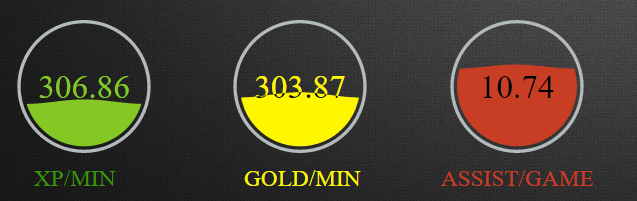
\includegraphics[width=0.5\textwidth]{indicators.png}
\caption{Gauge indicators of XP/MIN, GOLD/MIN and ASSISTS/GAME.}
 \label{Gauge}
 
\end{figure}


\begin{figure}
  \centering
  
    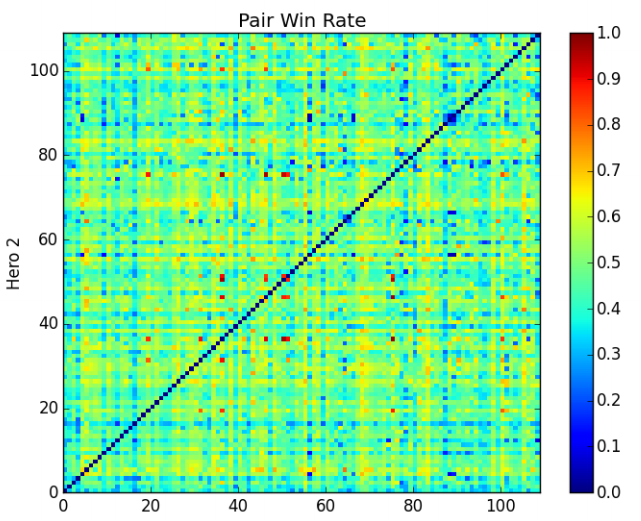
\includegraphics[width=0.5\textwidth]{stat.png}
\caption{Pairwise win rate with heatmap.[Win Prediction]}
 \label{heatmap}
 
\end{figure}

\section{DESIGN}
I think most of my effort was made to design part. To make Team Builder more convenient to use I tried many frameworks, visualization techniques, color and etc. My first idea was to visualize my project in edged graph form, but when I tried it, it become very messy and it was not very clear which edge corresponds to which heroes while there more than 100 heroes(Proposal design. Fig.~\ref{firstidea}). Since I was using vertexes' of graph as circle with hero's images and since it was really good-looking, I continued to use circles to later ideas as when representing objects and when making objects in ordered style. There 2 part of interface, first is hero choosing part, second is hero recommendation part.



\subsection{Hero Choosing}
In this interface (Fig.~\ref{herochoosing}) a user can choose a heroes for  enemy and ally team and can press start button to start computation of optimal hero and to go to another \emph{Hero Recommendation} interface. A 112 heroes are divided into 3 groups by their attributes. Each group is formed in circle-shape and each hero's image in group also shaped in circle form. On the left is located 'Strength' group, on the middle 'Intelligence' group and on the right is 'Agility' group. \emph{The main reason why I had chosen circle shaped style and divided into three groups because it was easier to find hero. Also each hero is zoom-able on hovering over.}



%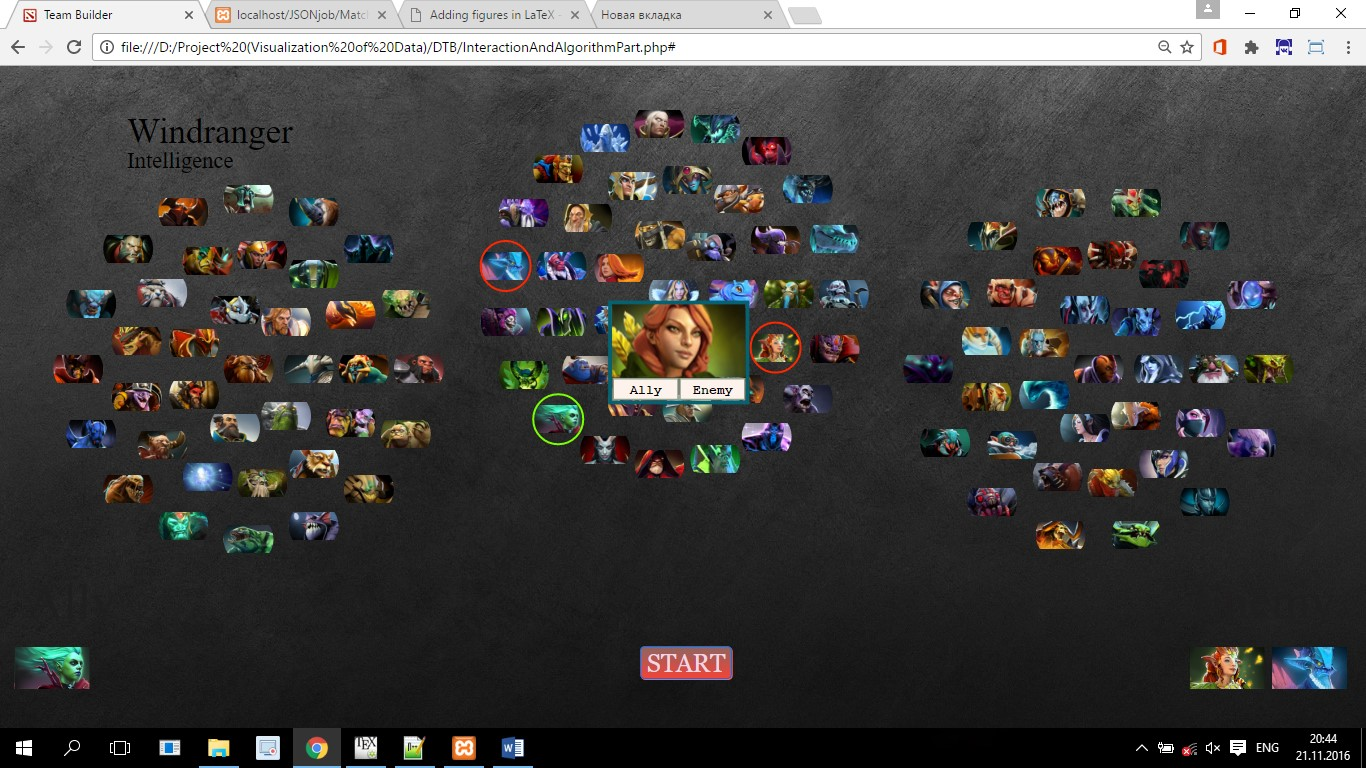
\includegraphics[width=90mm]{screen.png}

\begin{figure}
  \centering
  
    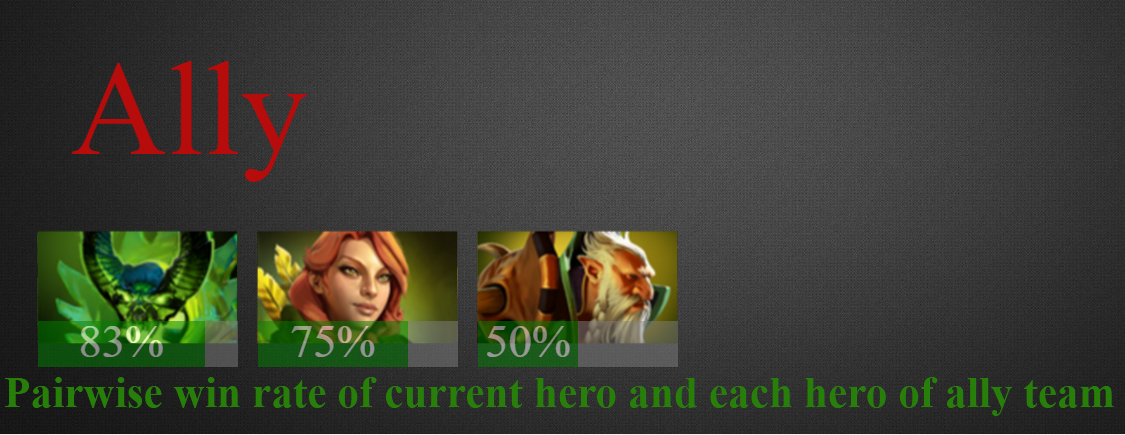
\includegraphics[width=0.5\textwidth]{Pairwise.png}
\caption{Pairwise win rate of between mousovered hero and ally team.}
 \label{pairwise}
 
\end{figure}







\subsection{Hero Recommendation}
This part (Fig.~\ref{recommendation}) helps a user to decide which hero will suit him/her best. There are 20 top optimal heroes given for a user to analyse them and select one of them. So the top 20 heroes are located on the center of page. They are located in such a way that the most optimal(which depends on the algorithm) is located in the center of all heroes and other heroes are laid on the edges of increasing circles. The bigger radius of hero, the more it is optimal. My visualization gives opportunity to gamer to see recommended heroes characteristics and ability to compare them and to choose the best hero which suits player. A user can compare heroes various characteristic by a stacked/grouped bar which is located on the left right  and animated indicator which allows a user to see an animated change in indicator which also help to see some differences between previous and current hero viewed. 


	1. \emph{Stacked/Grouped Bar} I used stacked bar to enable user to compare heroes with  comparable attributes of heroes and most effected to game results. There three values stacked in bar: 

		1) KILLS/DEATH [Top] - How good a hero kills. When a hero is a killer, he gains an experience and levels up fast which gives a more chance to win a game.
		
		2) WIN RATE[Mid] - How often hero wins. 

		3) PICK RATE[bottom] - How much hero is popular. Since most popular heroes known to each player, there is a big chance that ally team of user will know how to collaborate with chosen hero.

\emph{Stacked bar was used since all of these three attributes show the probability of wining the game and they can be added to give more precise results. Stacked bar can be easily transformed to grouped bar if a user wants to compare each of attributes individually(Fig.~\ref{grouped}).}


	2. \emph{Indicators} I used three gauge indicators to show heroes' three attributes:
			
		1)XP/MIN [Green] - How fast hero gains an experience
		
		2)GOLD/MIN [Yellow] - How fast hero collects gold
		
		3) ASSIST/GAME[Red] - How much a hero assists in killing enemy heroes 

\emph{I did not use any comparable framework, since these three attributes are almost incomparable. It means that it does not always bad or good if your XP/MIN is low or high, similarly for GOLD/MIN and ASSIST/GAME. But they give a user an information of how to play  with the hero with its full potential abilities. For example if a hero has high ASSIST/GAME, I can play with that hero as supporter hero (helping other heroes to attack) instead of being killer hero.}


There are two parts where a user can see why hovered hero was recommended:

\emph{1. It shows 'Good With' heroes, 'Good Against' heroes and 'Bad Against' heroes on the right center side. }
	
\emph{2.Under each ally heroes' images there pairwise green win rate indicators with mouseovered hero and under of each enemy heroes' image there win rate of mouseovered hero against enemy heroes(Fig.\ref{pairwise}).}

Select button gives a people chance to see hovered hero in ally team section and to start to compare new recommended heroes according their new generated data.

Back button gives ability to go to first interface part.

\emph{A user also can delete ally and enemy team heroes by clicking on image of heroes to see changes.}




 
  
					


										
												
\section{METHODS}
My approach for algorithm is dealing with relations between heroes and prioritizing heroes by numbers of 'bad relations' subtracted from 'good relations'. $priority = GR - BR$.

1. How did I compute it? Took all unselected heroes and for each of that heroes I counted number of 'Work' edges between ally team and number of 'Good' , 'Bad' edges for enemy team. Number of 'Work' edges considered as 'good relation' and 'Good' , 'Bad' edges are considered as 'bad relation'. Then I counted a priority from formula above.

2. Why this algorithm is said to be correct? As mentioned previously, a team is strong when heroes in team could function collectively by sharing their abilities.

Similarly to 'Win Prediction' paper I  used game data to compute pairwise win rate between each heroes and win rate of each hero against other heroes. For chosen ally team, I computed pairwise win rate of each ally hero with mouseovered hero and added result to $priority$. Similarly, I computed win rate of mouseovered hero against each hero in enemy team.
Now final priority equals to $$priorty = GR - BR + win_{with}+win_{against}$$

 \emph{Heatmap (Fig.~\ref{heatmap}) shows the win rate of team when $i_{th}$ hero and $j_{th}$ hero are played in that team. So we can see in this heatmap enough blue and red colors, it means that certain pair of heroes are not very compatible with each other and some are good when played in one team. So this experiment could strengthen our assumption by real results.}												

\begin{figure}
  \centering
  
    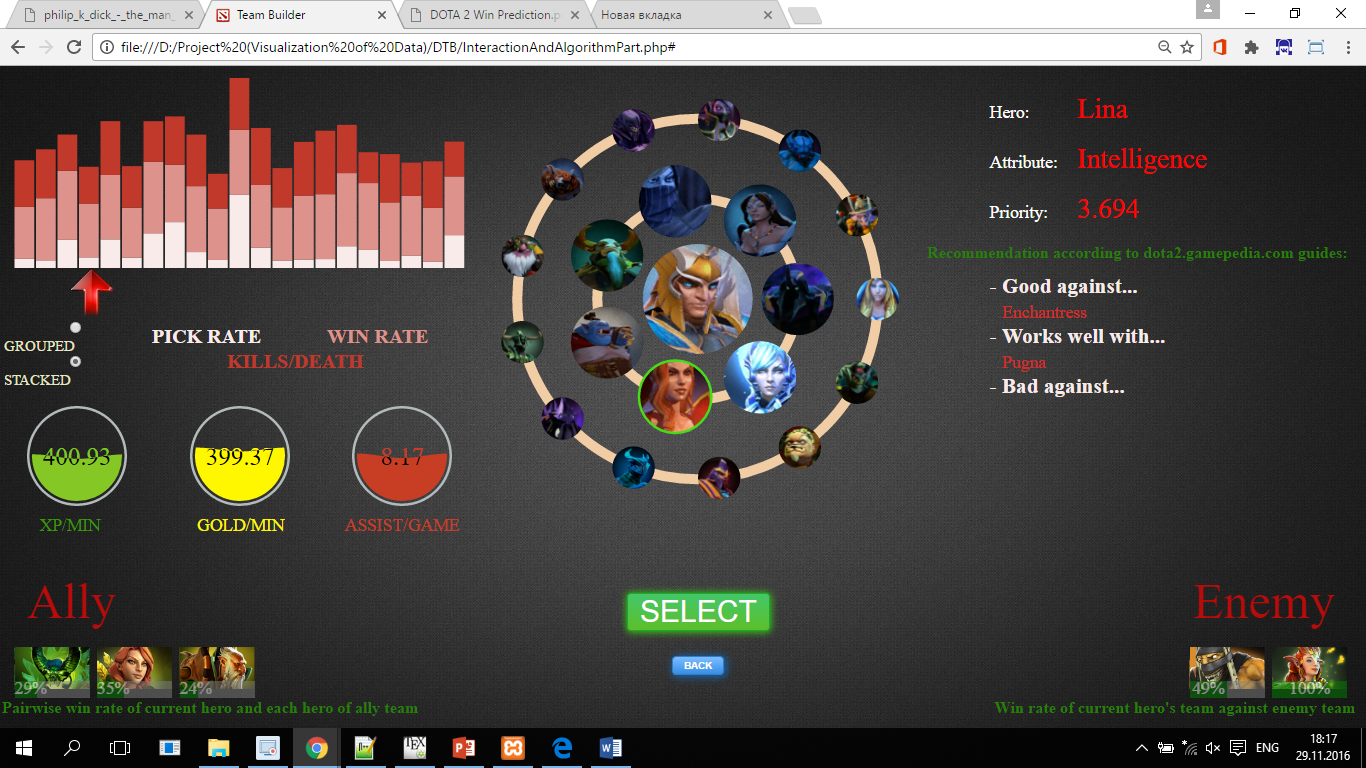
\includegraphics[width=0.5\textwidth]{recomendation.png}
\caption{Hero Recommendation part interface}
 \label{recommendation}
 
\end{figure}



							
											


\section{CONCLUSION}
Main purpose of Dota Team Builder to motivate users in reviewing their choice by comparing recommended heroes. Top 20 heroes lays out on the center which makes a user to focus on top heroes according their radius size. Stacked bar and gauge indicator frameworks were used to give a user information about current viewed hero. So DTB is not just a recommendation tool, it is also an interface for comparison heroes and information  about them.	





\section{FUTURE WORK}																			
I am intended to continue my work by adding to already existing data new game results to analyse more precisely. Since I do not see major problems in visualization part, I wanted to get feedbacks from users publishing it online. The algorithm also needs to be improved by machine learning algorithms as was offered in 'To win or not to win?' paper, since they are best solution for hero recommending know nowadays. 


\begin{thebibliography}{15}

\bibitem{Dotabase} 
Francis Tang. Alan Hsueh.							
\textit{Dotabase: a Dota 2 Database Visualizer}
	
\bibitem{Visualizing Match up Matrix} 
Cong Qiaoben
Stanford University						
\textit{Visualizing Match up Matrix}

\bibitem{To win or not to win? A prediction model to determine the outcome of
a DotA2 match
} 
Kaushik Kalyanaraman* Department of
Computer Science
University of California, San Diego\textit{To win or not to win? A prediction model to determine the outcome of
a DotA2 match
}
\bibitem{How}
How Does He Saw Me?
A Recommendation Engine for Picking Heroes in
Dota 2
\textit{Kevin Conley 
Daniel Perry.
Stanford University}
\bibitem{Prediction}
DOTA 2 Win Prediction
\textit{Nicholas Kinkade
Kyung yul Kevin Lim
University of California, San Diego
}

\bibitem{Prediction}
GAMEPEDIA 
\textit{\href{http://dota2.gamepedia.com/Dota_2_Wiki}{dota2.gamepedia.com}}
		
\bibitem{WEBAPI}
DOTA API
\textit{\href{https://wiki.teamfortress.com/wiki/WebAPI}{wiki.teamfortress.com}}


\end{thebibliography}

\end{document}